
\subsection{Predictions and early evidence for the quark gluon plasma}

Quantum chromodynamics (QCD) describes the interactions of the quarks and gluons (together known as partons) via the strong nuclear force.  The strength of the QCD interactions, described by the QCD coupling constant $\alpha_{s}(Q)$ decreases as distances between strongly interacting partons decreases and their exchanged momentum $Q$: 

\begin{equation}
\label{eq:alpha_s}
\alpha_{s}(Q) \propto \frac{1}{{\rm ln}(\frac{Q^{2}}{\Lambda_{QCD}})}, 
\end{equation}

\noindent where $\Lambda_{QCD} \approx 0.2$ GeV gives the QCD scale.  Figure~\ref{fig:alpha_s} shows the dependence of $\alpha_{s}$ on momentum scale $Q$.  In the regime where separations between partons are relatively large (small $Q$), $\alpha_{s}$ is large, leading to the observed confinement of quarks and gluons in composite particles called hadrons, most commonly baryons (comprised of 3 quarks, including protons and neutrons) and mesons (comprised of 2 quarks).  In the large $Q$ regime, however--accessed via large baryon chemical potential $\mu_{B}$ or large temperature $T$--the strength of the coupling constant $\alpha_{s}$ decreases, in a phenomenon known as asymptotic freedom.  Asymptotic freedom both permits the accurate approximation of high-energy hadron interactions using perturbation theory (pQCD), and implies the deconfinement of quarks and gluons.  This phase of deconfined quarks and gluons, known as the  quark gluon plasma (QGP), was originally conceived as a gas of color-charged quarks and gluons, analogous to the plasma of photons and electrons previously studied in quantum electrodynamics.  In collider studies, this suggests the possibility of a phase transition anticipated between the hadron gas phase present under ordinary matter conditions, and the QGP phase present at sufficiently great $\mu_{B}$ or $T$~\cite{Kalashnikov:1979, Shuryak:1980tp}.

\begin{figure}[h!]
\begin{center}
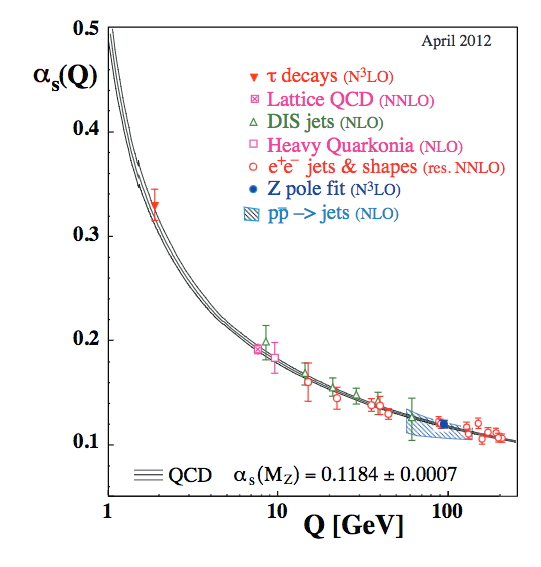
\includegraphics[width=0.6\textwidth]{figures/Theory/Alpha_s.png}
\caption[QCD coupling constant $\alpha_{s}$]{Momentum scale dependence of QCD coupling constant $\alpha_{s}$, from Ref.~\cite{Bethke:2012jm}.}
\label{fig:alpha_s}
\end{center}
\end{figure}


In the early 1980s, relativistic nuclear collisions were suggested as a means of producing sufficient temperatures and densities to induce a quark-gluon plasma and probe the transition between the QGP and ordinary matter.  Efforts were also made to anticipate key experimental signatures of the short-lived possible QGP, relying in many cases on the anticipation that the QGP would behave according to a hydrodynamic description of a system in at least partial thermal equilibrium.  Proposed signatures included enhancements of strange (heavy) quarks, unusual event structures, greater rates of direct dilepton and photon production~\cite{Bjorken:1983}.  The first heavy ion collisions began with fixed-target experiments at the Super Proton Synchrotron (SPS) at CERN in the mid-1980s, colliding nuclei including gold and lead at energies from 40 GeV to 160 GeV through the 1990s.  Analysis of the hadron yields in these collisions showed an apparent chemical equilibrium of quarks and gluons at about 170 MeV and enhancement (as anticipated) both of strangeness (via kaon/pion ratios, and J/$\psi$ production rates).  In the early 2000, a CERN press release cited these results in declaring that ``a common assessment of the collected data leads us to believe that a new state of matter has indeed been created...[that] features many of the characteristics of the theoretically predicted quark-gluon plasma''~\cite{Heinz:2000bk}.

Shortly after the SPS announcement, the first gold-gold collisions began at the Relativistic Heavy Ion Collider (RHIC) at Brookhaven National Laboratory, beginning an era of high-energy heavy ion collisions that would later be complimented by a parallel program at the Large Hadron Collider at CERN.  Through data collection and analysis by experiments at each of these colliders over the ensuing nearly two decades, the field has gradually shifted from searches for signatures of QGP formation in heavy ion collisions, to detailed characterizations of its properties and evolution.  In 2005, the four experimental collaborations at RHIC (BRAHAMS, PHENIX, PHOBOS, and STAR) published coordinated white papers~\cite{Arsene:2004fa, Adcox:2004mh, Back:2004je, Adams:2005dq} summarizing the assembled evidence that results from  gold-gold collisions could not be explained by models of ordinary hadronic matter--most notably in signatures of collective behavior (see Sec.~\ref{sec:theory_collectivity}) and in suppression of particles with relatively high transverse momentum (see Sec.~\ref{sec:theory_jets}).  Beginning in 2010, heavy ion studies at the LHC by the ALICE, ATLAS, and CMS Collaborations (and more recently by the LHCb Collaboration) have complimented the RHIC access to a wide range of center-of-mass-energies in the 7.7 GeV to 200 GeV range with measurements at 2.76 TeV and 5.02 TeV.

\subsection{Properties of the quark gluon plasma}

-- Temperature and energy density at RHIC and LHC energies

-- Time-evolution (initial conditions, hydrodynamic expansion of the QGP, hadronization)

-- QCD phase diagram characterization

\subsection{Characterizing collision centrality}
\label{sec:glauber}

-- Glauber model

***** GLAUBER DIAGRAM *****

-- TAA

-- Glauber limitations

-- Experimental definitions of centrality


\subsection{Collective behavior in the QGP}
\label{sec:theory_collectivity}

-- Flow and interpretations (including harmonic decomp. examples)

-- Hydro

-- IS fluctuations

***** DIAGRAM OF IS CONFIGURATIONS AND CONNECTION TO HARMONICS******

\clearpage

\section{Jets as probes of the quark gluon plasma}
\label{sec:theory_jets}

Hard scatterings in heavy ion collisions can provide powerful $in situ$ probes of the quark gluon plasma.  Because of asymptotic freedom, high-energy parton-parton processes can be accurately characterized via pQCD, and have been thoroughly studied experimentally in hadron-hadron collisions.  In heavy ion collisions, the initial parton-parton interaction should by 
causality behave the same as a parton-parton interaction in hadron-hadron collisions.  After the collision, however, outgoing partons traverse the quark gluon plasma, providing the opportunity to study medium properties by comparing heavy ion results to expectations inferred from hadron-hadron ``vacuum'' reference data.  These studies are facilitated by the ``factorization theorem'' in pQCD, which states that the cross section $\sigma_{AB\rightarrow h}^{\rm hard}$ of hadron $h$  produced in the hard process $ A + B \rightarrow h$) can be decomposed into contributions from:  

\begin{itemize}
\item The perturbative cross section of the parton hard scattering $\sigma_{ab\rightarrow c}^{\rm hard}$ 
\item The initial parton distribution functions (PDFs) of partons in the colliding nuclei A and B ($f_{a/A}$ and $f_{b/B}$ for partons of flavor $a$ and $b$)
\item The fragmentation function $\mathscr{D}_{c\rightarrow h}$ describing the probability that parton $c$ fragments into hadron h with momentum fraction $z = p_{h}/p_{c}$ 
\end{itemize}

\noindent The total cross section may be represented, schematically, as:  

\begin{equation}
\label{eq:factorization}
d \sigma_{AB\rightarrow h}^{\rm hard} = f_{a/A}(x_{a},Q^{2})  f_{b/B}(x_{b},Q^{2}) \times d \sigma_{ab\rightarrow c}^{\rm hard}(x_{a},x_{b},Q^{2}) \times \mathscr{D}_{c\rightarrow h}(z,Q^{2}),
\end{equation}

\noindent Each contribution to $d \sigma_{AB\rightarrow h}$ can be experimentally determined, and in hadron-hadron collisions $\sigma_{ab\rightarrow c}^{\rm hard}$, fragmentation functions, and PDFs should each be universal.  The partonic cross section $\sigma_{ab\rightarrow c}^{\rm hard}$ furthermore should not, by causality, depend on the presence or absence of the QGP.  Medium modifications may enter at two phases in this process:  first, via energy loss by parton $c$ passing through the medium, and second via possible medium-induced changes to fragmentation functions $\mathscr{D}_{c\rightarrow h}$.  Parton energy loss is attributed to two primary mechanisms:  collisional energy loss from scatterings with partons in the medium, and medium induced radiation roughly analogous to electromagnetic ionization in a medium~\cite{Bjorken:1982tu, d'Enterria:2009am}.  

**** DIAGRAM OF FACTORIZATION WITH QGP MODIFICATIONS NOTED ****

This medium-induced parton energy loss implies an observable reduction of Medium properties can also be further probed by comparing measurements of jet substructure in heavy ion collisions compared to pp reference data (Sec.~\ref{sec:jff_jetshapes}), and by studying modifications to $p_{\rm T}$ balance in back-to-back dijet events (Sec.~\ref{sec:dijet_balance}).


\subsection{Measuring suppression of high-$p_{\rm T}$ particles and jets}
\label{sec:raa}

One observable to probe parton energy loss in the medium is to compare yields of both particles with relatively high transverse momentum ($p_{\rm T}$), and of reconstructed jets (collections of particles clustered in an effort to reconstruct the original parton energy -- see Sec.~\ref{sec:Jets}).  This reduction in jet yields compared to expectations from ``vacuum'' reference or scaled binary collisions can be studied as both a signature of the presence of the QGP, and an observable to distinguish between models of interactions within the QGP (see Sec.~\ref{sec:raa}).  

Since by pQCD factorization the partonic cross-section $\sigma_{ab\rightarrow c}$ should be independent, in the absence of the quark gluon plasma, the nuclear inclusive cross section would be expected to scale with the number of participating nucleons, i.e.  

\begin{equation}
\label{eq:raa_p0}
d \sigma_{AB\rightarrow h}^{\rm hard}(b) = \langle T_{AB}(b) \rangle \sigma_{pp}^{\rm hard}
\end{equation}

\noindent where $T_{AB}(b)$ parameterizes the probability of nucleon-nucleon interactions for a given impact parameter for nucleii A and B colliding with impact parameter $b$ as discussed in Sec.~\ref{sec:glauber}.  A comparison of actual hadron (or jet) yields compared to this expectation can therefore give information about parton interactions with the medium, as characterized by the nuclear modification factor $R_{AA}$ defined as the ratio of the observed yield in heavy ion data to the expecation from binary scaled pp data: 

\begin{equation}
\label{eq:raa_trk}
R_{AA}(p_{\rm T}, \eta) = \frac{d^{2}\sigma_{AA}/dp_{\rm T} d\eta}{\langle T_{AB}(b) \rangle  d^{2}\sigma_{pp}/dp_{\rm T} d\eta},
\end{equation}

Consistent with quenching expectations, RHIC measurements of $R_{AA}$ in gold-gold collisions showed substantial suppression of a factor of 70-80\% for $p_{\rm T} > 4$ GeV~\cite{Arsene:2004fa, Adcox:2004mh, Back:2004je, Adams:2005dq}.  Comparisons of RHIC measurements to early LHC results showed similar qualitative features, but greater suppression at low-$p_{\rm T}$ at the LHC, despite the more slowly falling pp spectrum at the LHC, as shown in Fig.~\ref{fig:alice_chpart_raa}.  Measurements at the LHC have also found that $R_{AA}$ rises with $p_{\rm T}$ for charged particles with $p_{\rm T} > 7$ GeV, and have shown no significant center-of-mass energy differences when comparing $R_{AA}$ at 2.76 TeV and 5.02 TeV, as shown in Fig.~\ref{fig:cms_chpart_raa}.  The $p_{\rm T}$ dependence of $R_{AA}$ is generally driven by three factors:  the kinematic constraints on jet energy loss (model-specific details will be discussed in Sec.~\ref{sec:theory_models}), the fact that $R_{AA}$ takes the ratio of two steeply falling spectra the scattered partons, one shifted by energy loss and one un-shifted, and the effects of nuclear shadowing and anti-shadowing in the nuclear PDFs.~\cite{d'Enterria:2009am, Armesto:2006ph}

\begin{figure}[h!]
\begin{center}
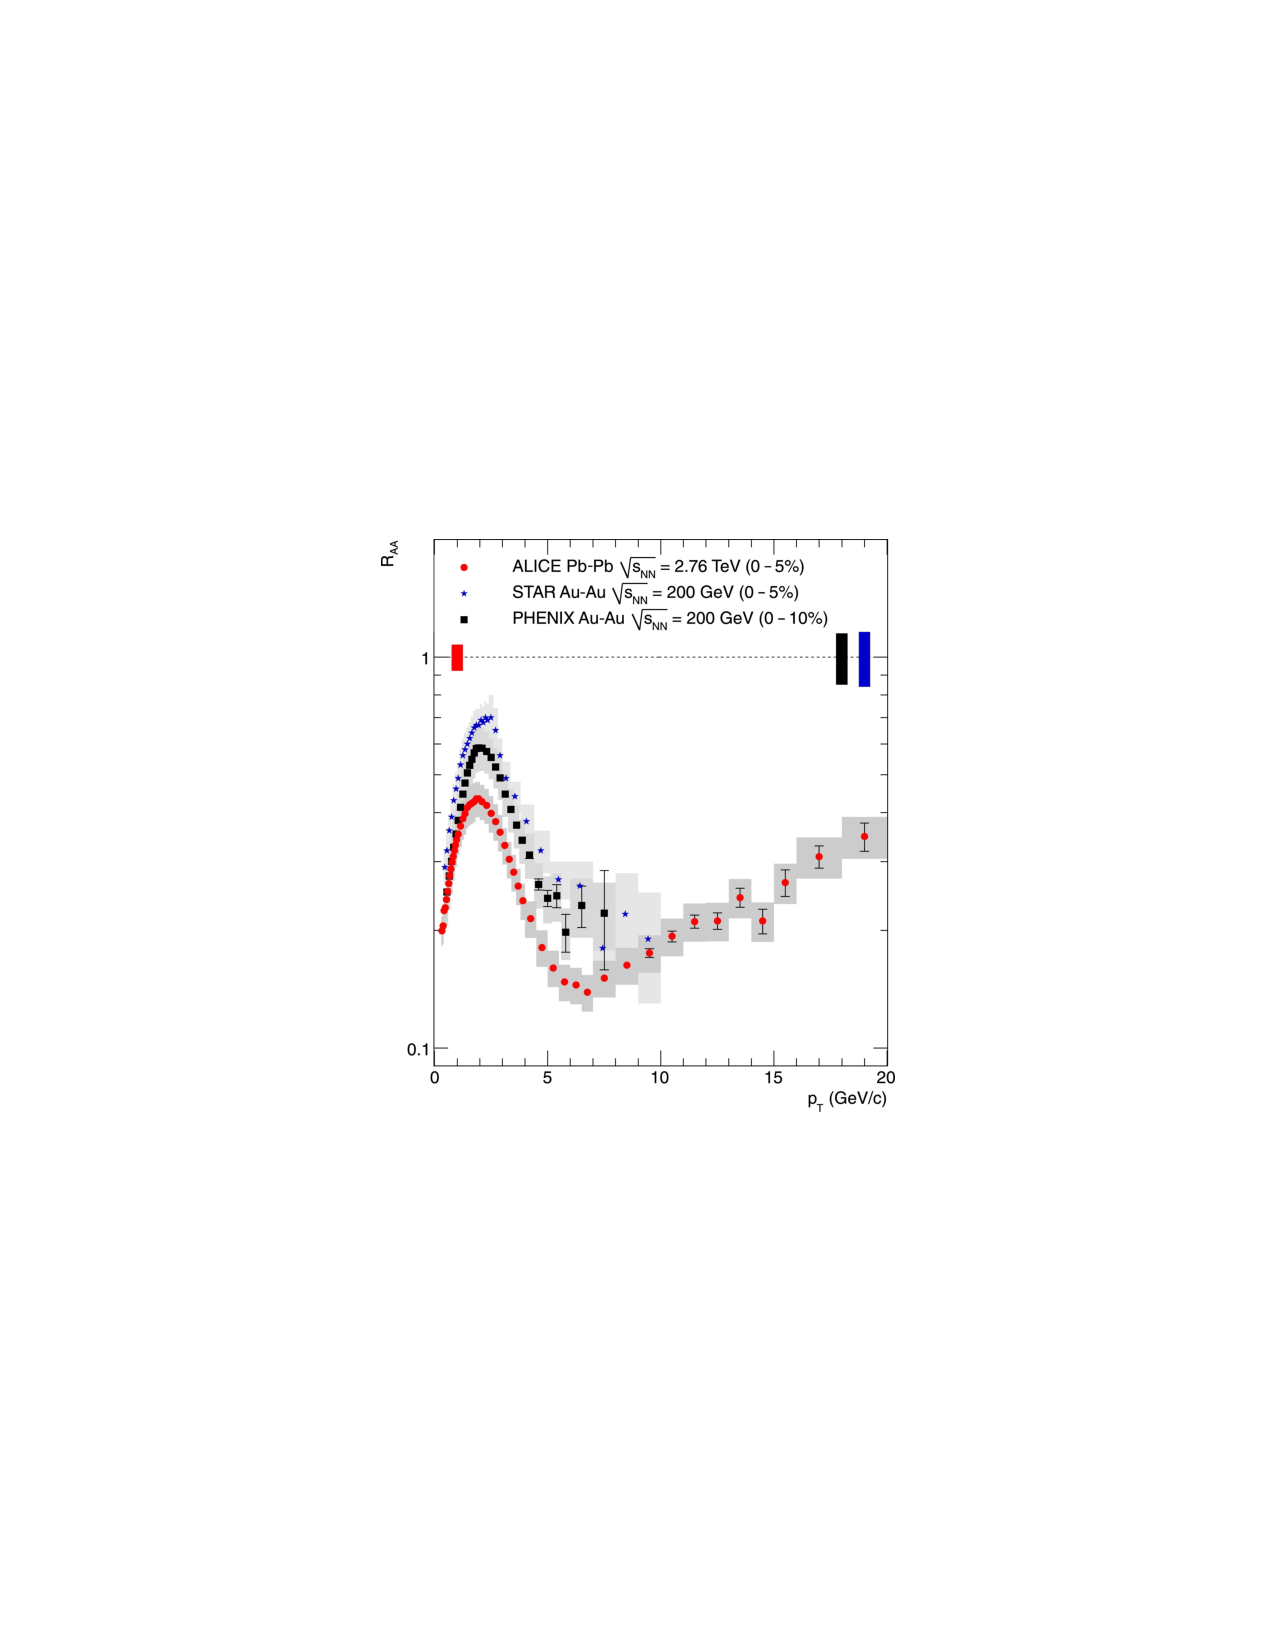
\includegraphics[width=0.7\textwidth]{figures/Theory/ChPart_Raa_ALICE_RHIC.pdf}
\caption[Charged particle $R_{AA}$ at 200 GeV and 2.76 TeV]{Measurements of charged particle $R_{AA}$ from the STAR and PHENIX Collaborations at 200 GeV at RHIC, compared to ALICE results from the LHC at 2.76 TeV from Ref.~\cite{Aamodt:2010jd}.}
\label{fig:alice_chpart_raa}
\end{center}
\end{figure}

\begin{figure}[ht!]
\begin{center}
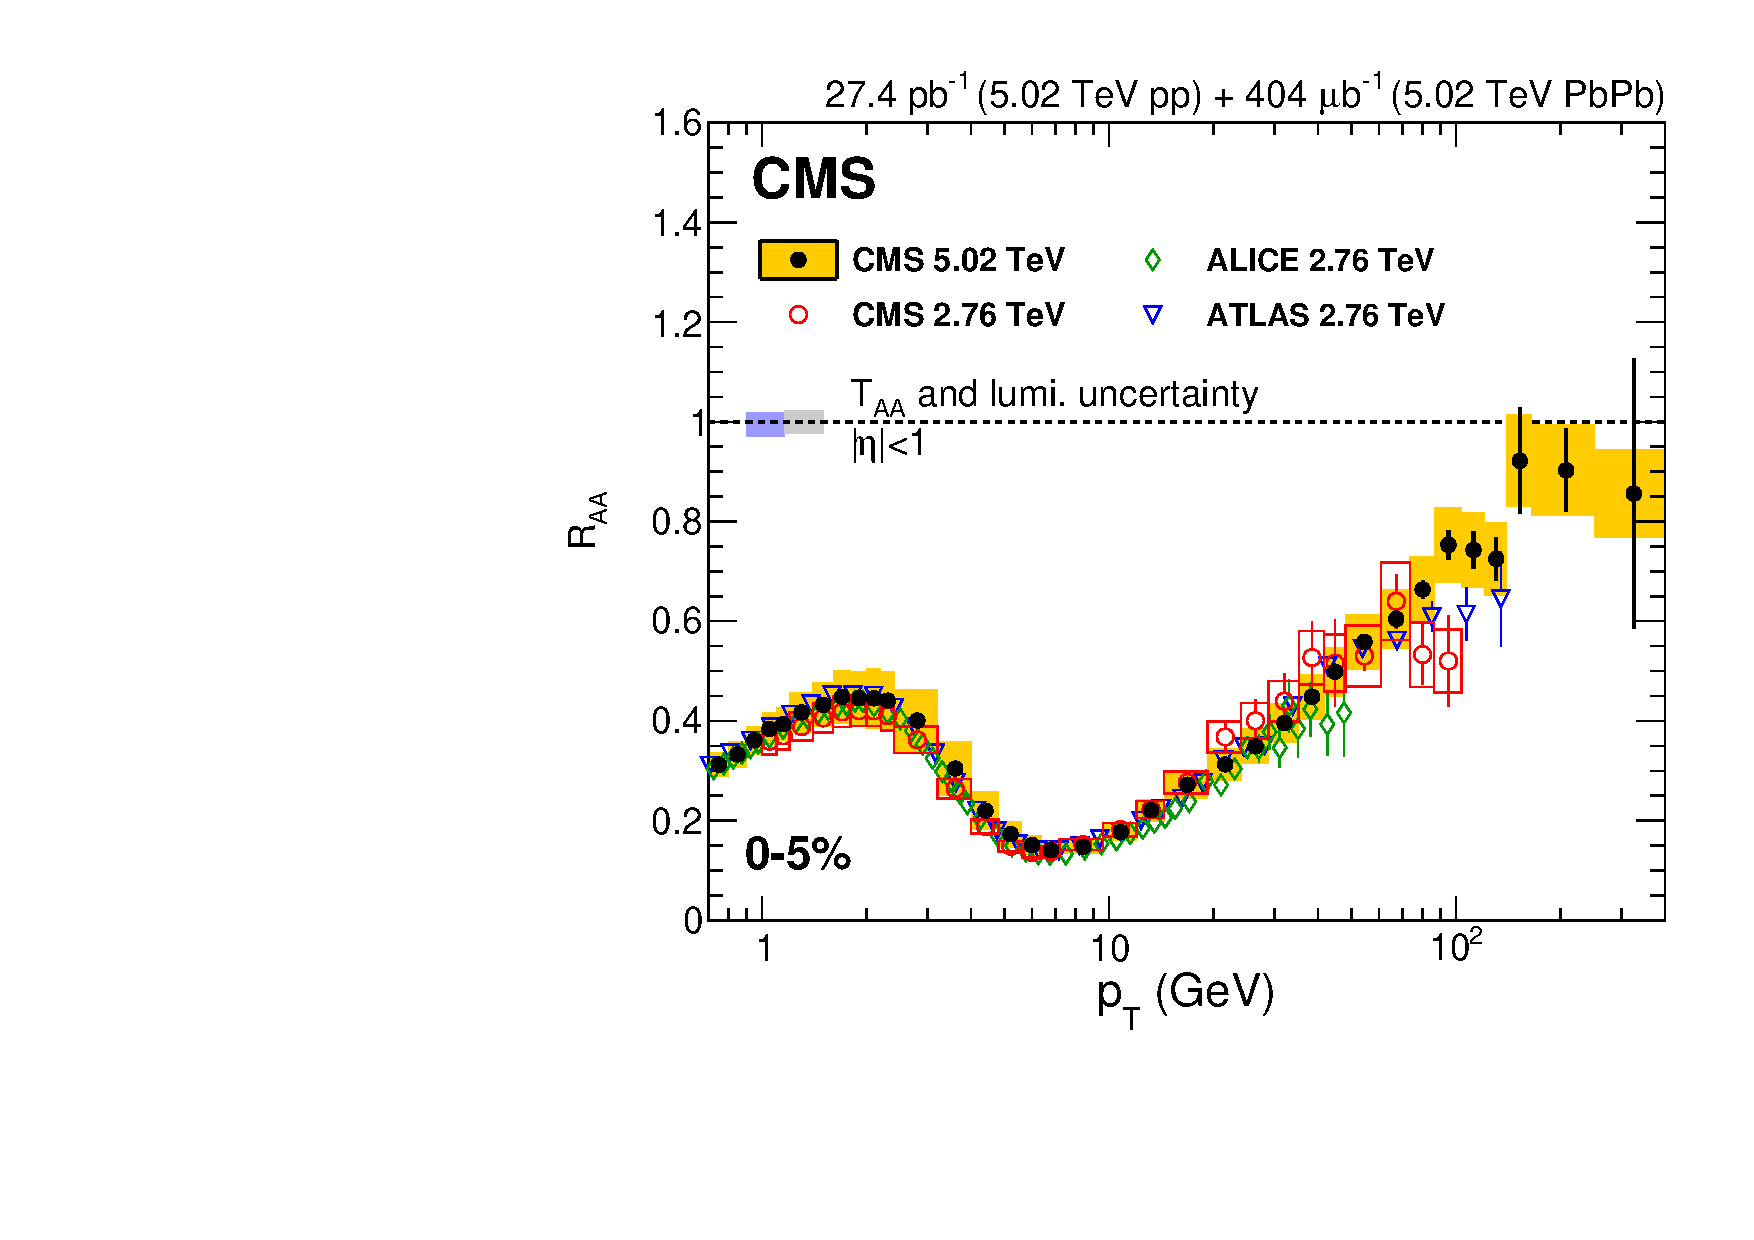
\includegraphics[width=0.7\textwidth]{figures/Theory/ChPart_Raa_CMS_LHC.pdf}
\caption[Charged particle $R_{AA}$ at 2.76 and 5.02 TeV]{Measurements of charged particle $R_{AA}$ at LHC energies 2.76 TeV and 5.02 TeV from Ref.~\cite{Khachatryan:2016odn}.}
\label{fig:cms_chpart_raa}
\end{center}
\end{figure}


Studies of high-$p_{\rm T}$ tracks make use of the fact that such tracks are likely to originate from outgoing partons in hard-scattering interactions, providing an indirect look at energy loss by the parton used as a probe of the QGP.  To more directly reconstruct parton energy, we may instead consider reconstructed jets, defined as the collection of (spatially grouped) particles resulting from the fragmentation of a high-$p{\rm T}$ quark or gluon.  Jet reconstruction, described in detail in Sec.~\ref{sec:Jets}, groups detector deposits to reconstruct a jet energy, and uses Monte Carlo simulation to reconstruct a ``true'' jet energy of the original parton. 

***** DIAGRAM OF WHAT IS A JET *****

Quenching studies with reconstructed jets therefore can offer a more direct look at energy loss in the medium by comparing measured energy in jets in heavy ion collisions to those in proton-proton collisions.  Measurements of jet $R_{AA}$ at the LHC reported in Refs.~\cite{Aad:2014bxa, Khachatryan:2016jfl} show suppression by a factor of approximately 40-60\% in most central PbPb collisions, with weak depenence on jet $p_{\rm T}$ as shown in Fig.~\ref{fig:cms_jet_raa}.  

\begin{figure}[h!]
\begin{center}
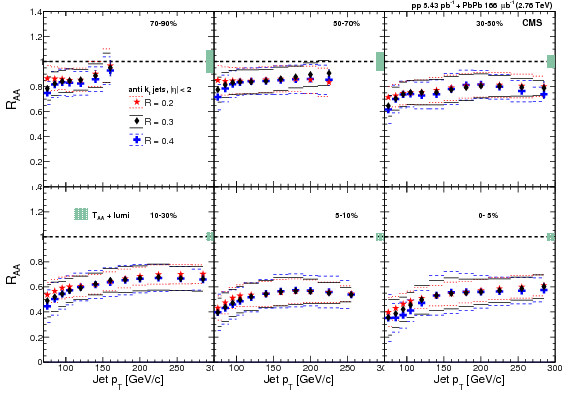
\includegraphics[width=0.99\textwidth]{figures/Theory/JetRaa_CMS.png}
\caption[Jet $R_{AA}$ at 2.76 TeV]{Jet $R_{AA}$ at 2.76 TeV from Ref.~\cite{Khachatryan:2016jfl}.}
\label{fig:cms_jet_raa}
\end{center}
\end{figure}


Jet $R_{AA}$ measurements capture parton energy loss by measuring the reduction in yields in the presence of the QGP.  To connect jet $R_{AA}$ to charged particle $R_{AA}$ measurements, it is necessary to also consider trends in jet fragmentation patterns with jet-$p_{\rm T}$.  High-$p_{\rm T}$ jets are more likely to originate from quarks than from gluons, and therefore exhibit ``harder'' fragmentation patterns--i.e. higher-$p_{\rm T}$ jets fragment into relatively fewer particles each with more $p_{\rm T}$ compared to jets at lower-$p_{\rm T}$.  Jets with softer fragmentation are also expected to exhibit greater modification in the QGP, as low-$p_{\rm T}$ fragmentation products rescatter in the medium.  The highest-$p_{\rm T}$ tracks, for which $R_{AA}$ is the smallest, are associated with those jets that have not only the highest-$p_{\rm T}$, but also the hardest fragmentation.  The high-$p_{\rm T}$ sector of jet $R_{AA}$ measurements at LHC energies, however, still includes significant contributions from jets reconstructed from softer particles that exhibit significant suppression.

\clearpage

\subsection{Jet fragmentation function and jet shape measurements}
\label{sec:jff_jetshapes}

Measurements of jet $R_{AA}$ quantify the overall reduction in numbers of high-$p_{\rm T}$ jets passing a certain momentum threshold, providing an indication of the magnitude of jet energy loss in different $p_{\rm T}$ regions.  As discussed above, this measurement can constrain the possible mechanisms of jet energy loss.  To further constrain models of jet energy loss, additional observables aim to capture the details of jet fragmentation and its modification in the quark gluon plasma.  One such measurement is the jet fragmentation function, which captures the $p_{\rm T}$ distribution of tracks carying jet momentum, paramaterized via the variables $z$ and $\zeta$: 

\begin{equation}
\label{eq:jff_cms}
z = \frac{p^{\rm track}_{\rm ||}}{p^{\rm jet}_{\rm ||}}, \zeta = \frac{1}{{\rm ln} (z)},
\end{equation}

\noindent where $p^{\rm track}_{\rm ||}$ refers to the component of the track $p_{\rm T}$ along the jet axis.  Jet fragmentation function measurements from CMS shown in Fig.~\ref{fig:cms_jff} show a centrality-dependent modification to fragmentation function in PbPb relative to pp data, with a depletion in the mid-$\zeta$ range, balanced by an enhancement at large $\zeta$, in the region corresponding to low-$p_{\rm T}$ tracks.  This shows a redistribution of energy within the jet cone toward softer particle production in the presence of the medium, consistent with predictions of parton energy loss corresponding to a suppression of high-$p_{\rm T}$ particles (model details will be discussed in Sec.~\ref{sec:theory_models}).

\begin{figure}[h!]
\begin{center}
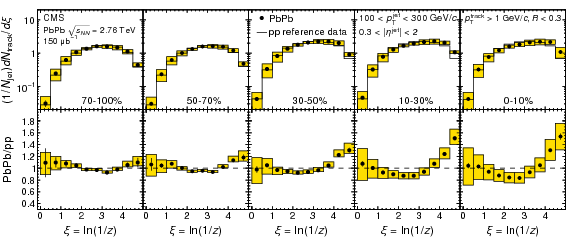
\includegraphics[width=0.99\textwidth]{figures/Theory/CMS_JFF.png}
\caption[Jet fragmentation function in 2.76 TeV PbPb and pp data]{Jet fragmentation function for jets with $100 < p_{\rm T} < 300$ GeV in 2.76 TeV PbPb and pp data from Ref.~\cite{CMS:2012vba}.}
\label{fig:cms_jff}
\end{center}
\end{figure}

In addition to characterizing the $p_{\rm T}$ spectrum of jet constituents, the distribution of $p_{\rm T}$ with respect to the jet axis can also help to constrain fragmentation scenarios.  This distribution, known as the jet shape, is defined within the jet cone as: 

\begin{equation}
\label{eq:jet_shape_cms}
\rho(\Delta r) = \frac{1}{\delta r}\frac{1}{N^{\rm jet}} \mathlarger{ \sum \limits_{\rm jets}} \frac{\Sigma_{{\rm tracks}\in[r_{a},r_{b})} p_{\rm T}^{\rm track}}{p_{\rm T}^{\rm jet}},
\end{equation}

\noindent where $r_{a}$ and $r_{b}$ correspond to the inner and outer radii, respectively, of an annulus of width $\delta r = 0.5$ around the jet axis.  The first jet shape measurement from CMS, shown in Fig.~\ref{fig:cms_jet_shape} (measured with particles with $p_{\rm T} > 1$ GeV), shows a spatial redistribution of energy from small radii ($\Delta r \approx 0.1$) to larger radii ($\Delta r > 0.2$) from the jet axis.  This is qualitatively consistent with predictions of energy redistribution into particles that are both relatively soft ($p_{\rm T} < 3 $ GeV, as observed in jet fragmentation function measurements), and recovered at relatively large angles from the jet axis.  In this way, the study of jet shape modifications $within$ the jet cone motivate extension of these measurements to larger angles from the jet axis to quantify the distribution and $p_{\rm T}$ composition of particles at angles larger than $\Delta r = 0.3$.  

\begin{figure}[hbtp]
\begin{center}
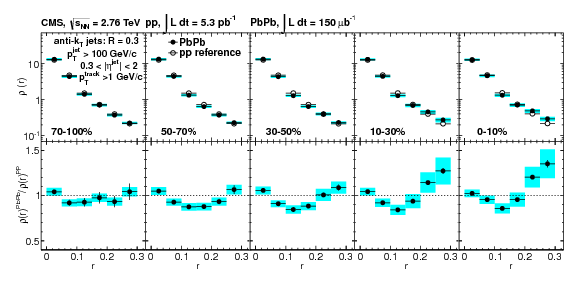
\includegraphics[width=0.99\textwidth]{figures/Theory/CMS_JetShapes.png}
\caption[Jet shape measurement in 2.76 TeV PbPb and pp data]{Jet shape measurement in 2.76 TeV PbPb and pp data from Ref.~\cite{Chatrchyan:2013kwa}.}
\label{fig:cms_jet_shape}
\end{center}
\end{figure}


\clearpage 

\subsection{Dijet asymmetry and momentum balance studies}
\label{sec:dijet_balance}

Additional possibilities for exploration of medium properties follow from the consideration of ``dijets,'' jets that are back-to-back in azimuthal angle ($\Delta \phi_{\rm jets} \approx \pi$).  As the incoming collision participants each begin with $p_{\rm T} \approx 0$ GeV, the total $p_{\rm T}$ of outgoing partons immediately after the collision must also be 0.  If both partons experience either no energy loss (as in the vacuum) or approximately equal energy loss (i.e. by experiencing roughly equal path-lengths through the medium), the measured $p_{\rm T}$ of each jet in the dijet pair would be approximately equal.  If, however, the hard-scattering occurs toward the surface of the QGP, the jet with a longer path-length through the medium might be expected to experience substantially more energy loss, leading to a $p_{\rm T}$ asymmetry in the dijet pair.  This expectation was probed via studies of di-hadron correlations with high-$p_{\rm T}$ particle triggers ($4 < p_{\rm T} < 6$ GeV by STAR at RHIC, $8 < p_{\rm T} < 15 $ GeV by ALICE at the LHC) showed results consistent with the expectation.  These studies showed the substantial suppression (even disappearance, in the STAR studies) of yields of particles with $p_{\rm T} > 2$ GeV in the region opposite the trigger hadron in azimuth~\cite{Adler:2002tq, Aamodt:2011vg}, consistent with path-length dependent jet quenching and a surface bias in trigger particles.  

***** DIAGRAM OF UNBALANCED DIJETS *****

The large kinematic reach of hard probes at the LHC allows for dijet studies at much higher $p_{\rm T}$.  The first of these studies measured the ``dijet imbalance'' between the highest-$p_{\rm T}$ (``leading jet,'' with $p_{\rm T,1}$) and second-highest-$p_{\rm T}$ jets (``subleading jet,'' with $p_{\rm T, 2}$ in the event, parameterized as: 

\begin{equation}
\label{eq:aj}
A_{\rm J} = \frac{p_{\rm T,1} - p_{\rm T,2}}{p_{\rm T,1} + p_{\rm T,2}}
\end{equation}

\noindent These studies, by the ATLAS and CMS Collaborations~\cite{Aad:2010bu, Chatrchyan:2011sx} showed a centrality-dependent shift in the $A_{\rm J}$ in PbPb collisions, with greater dijet asymmetry in central PbPb data than in pp or in peripheral PbPb collisions.  In pp and peripheral PbPb collisions, asymmetric dijet events are those in which some $p_{\rm T}$ is carried by a third jet, and the $A_{\rm J}$ distribution is steeply falling.  In central PbPb collisions, however, there are expected to be two contributions to the sameple of asymmetric dijet events: not only three-jet events, but also dijet events in which the subleading jet is substantially quenched.  As shown Fig.~\ref{fig:cms_dijets}, this effect is evident in the shift toward larger values of $A_{\rm J}$ in central PbPb collisions. 

\begin{figure}[hbtp]
\begin{center}
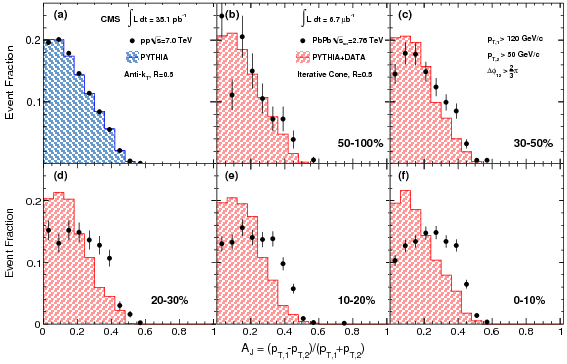
\includegraphics[width=0.9\textwidth]{figures/Theory/CMS_dijets.png}
\caption[Dijet asymmetry and in 2.76 TeV PbPb and pp data]{Dijet asymmetry in 2.76 TeV PbPb and pp data for jet selection $p_{\rm T,1} > 120$ GeV, $p_{\rm T,2} > 50$ GeV, and $\Delta\phi_{\rm 1,2} > 2\pi/3$ from Ref.~\cite{Chatrchyan:2011sx}.}
\label{fig:cms_dijets}
\end{center}
\end{figure}

The transverse momentum difference between the leading and subleading jets may be conceptualized as ``missing-$p_{\rm T}$'' from the subleading jet, which must by momentum conservation be recovered somewhere in the hemisphere of the event surrounding the subleading jet axis.  One way to capture this momentum balance is by comparing the total $p_{\rm T}$ carried by tracks in different $p_{\rm T}$ classes in the subleading relative to the leading hemisphere.  This balance is shown in the top row Fig.~\ref{fig:cms_mpT}, for $\slashed{p}_{\rm T}^{\rm ||}$ defined as the projection of each track's $p_{\rm T}$ projected in $\phi$ onto the dijet axis (i.e. the average of the leading and subleading jet axes)~\ref{HIN_2014_010}.  In pp and peripheral PbPb data, this balance shows the depletion of tracks with $p_{\rm T} > 8$ GeV in the subleading relative to the leading hemisphere balanced primarily by tracks with $2 < p_{\rm T} < 8$ GeV, consistent with the localization of these tracks in additional jets for unbalanced dijets in this scenario.  The magnitude of the ``missing-$p_{\rm T}$'' balancing distribution increases with growing $A_{\rm J}$ by construction.  Comparing PbPb to pp distributions (differences shown int he bottom row of Fig.~\ref{fig:cms_mpT}), the balancing distribution in unbalanced (large $A_{\rm J}$) events in central PbPb data shows larger contributions from soft particles with $p_{\rm T} < 2$ GeV and smaller contributions from particles with $p_{\rm T} > 4$ GeV, indicating that the more of the balancing $p_{\rm T}$ distribution in the subleading side is carried by soft quenching products rather than additional jets. 


\begin{figure}[hbtp]
\begin{center}
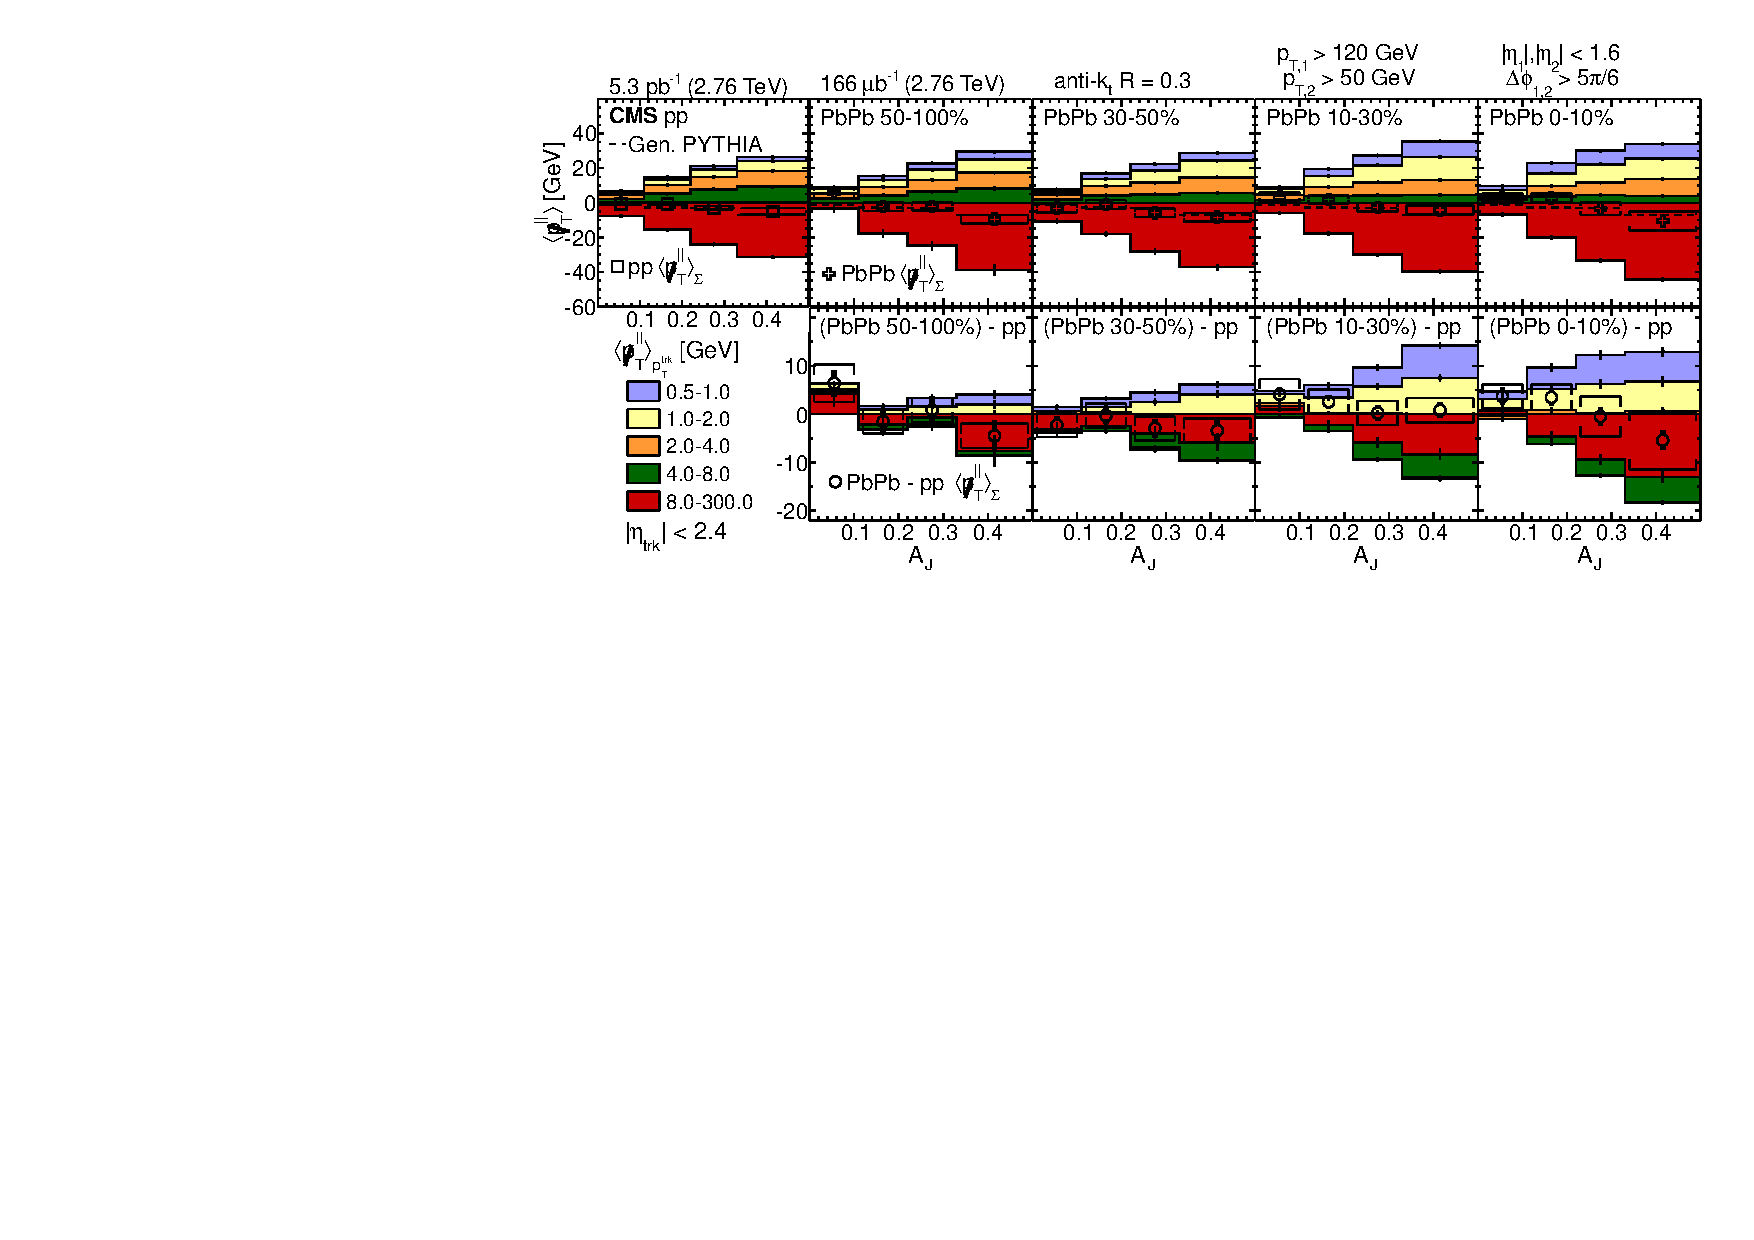
\includegraphics[width=0.99\textwidth]{figures/Theory/CMS_mpT.pdf}
\caption[Hemisphere $p_{\rm T}$ momentum balance in dijet events as a function of $A_{\rm J}$]{Top row: hemisphere $p_{\rm T}$ momentum balance in dijet events as a function of $A_{\rm J}$, taking the total difference $\slashed{p}_{\rm T}^{\rm ||}$ in the subleading hemisphere minus that in the leading hemisphere from Ref.~\ref{HIN_2014_010} in pp and PbPb data.  Bottom row:  Differences PbPb - pp.}
\label{fig:cms_mpT}
\end{center}
\end{figure}

Dijet momentum balance studies therefore show evidence of redistribution of jet energy from harder to softer particles via jet quenching, and greater quenching of the subleading than leading jets.  As discussed above, the angular distribution of quenching products relative to the jet axis is also highly relevant for constraining models of interactions between the jet and the medium.  This measurement is shown in Fig.~\ref{fig:cms_mpT_unbalanced} for unbalanced dijets with $A_{\rm J} > 0.22$.  Comparing the radial distribution with respect to the dijet axis shows that in this unbalanced dijet sample in central PbPb events, more $p_{\rm T}$ is recovered in lower-$p_{\rm T}$ particles extending to large angles from the jet axis.  It is important to note that this measurement shows overall hemisphere differences in the radial $p_{\rm T}$ distribution, combining the effects of quenching to the subleading jet, quenching to the leading jet, and also any azimuthal asymmetry in the underlying event (as would arise if the direction of the dijet axis coupled to odd underlying event flow terms such as $v_{\rm 3}$).  Isolating and further studying each of these contributions will be a major goal of this analysis, as discussed in Sec.~\ref{sec:motivation_decomp}.


\begin{figure}[hbtp]
\begin{center}
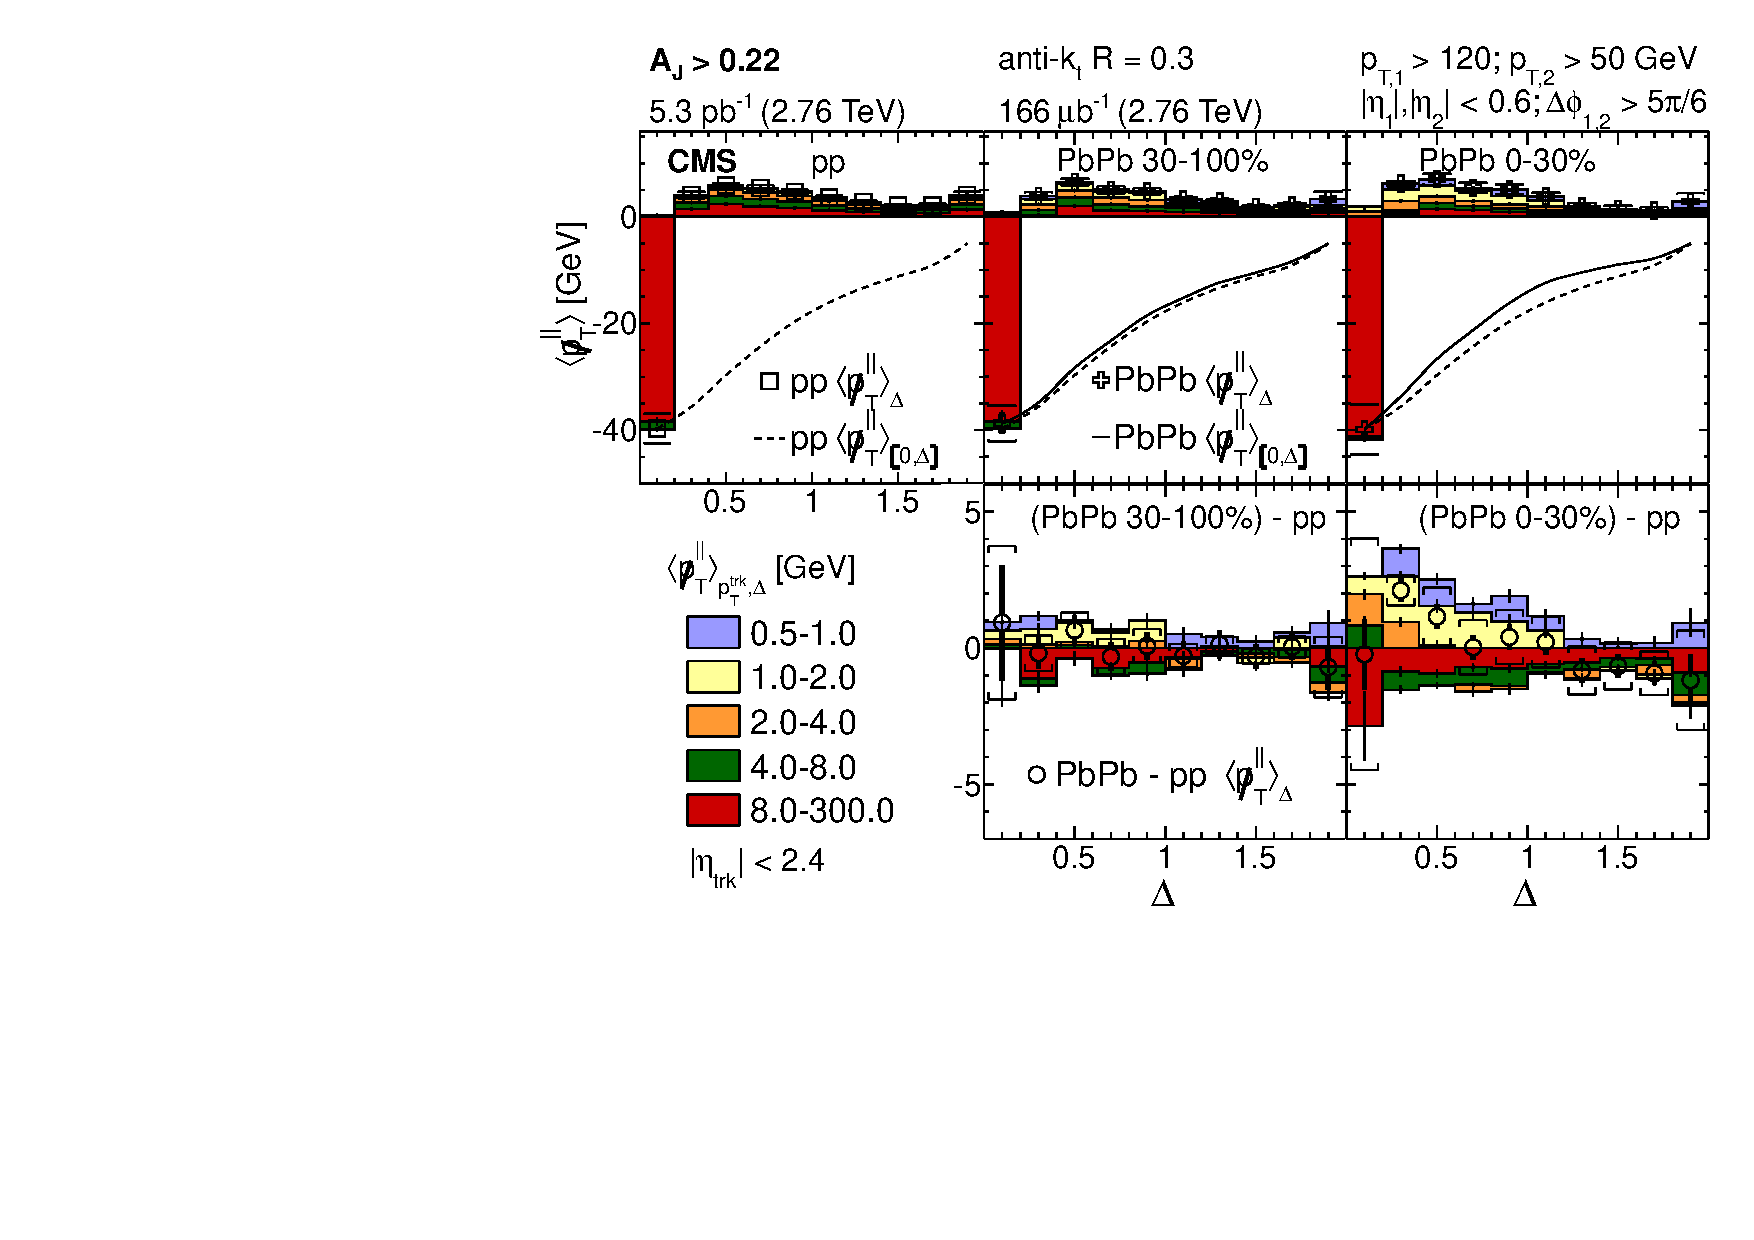
\includegraphics[width=0.9\textwidth]{figures/Theory/MpT_Unbalanced.pdf}
\caption[]{}
\label{fig:cms_mpT_unbalanced}
\end{center}
\end{figure}




\clearpage


\section{Models of jet energy loss in the quark gluon plasma}
\label{sec:theory_models}

A range of theoretical models of jet quenching have been developed to specifically account for the energy loss of a propagating probe through the quark gluon plasma.  In general, models characterize collisional energy loss mechanisms (i.e. jet energy loss via elastic interactions with the medium), radiative energy loss by the propagating parton, and in some cases a medium response in the form of a ``plasma wave'' or back reaction.  Some prominent examples of specific quenching models are surveyed briefly in Sec.~\ref{sec:model_survey}.  Some relevant comparisons to data are shown in Sec.~\ref{sec:model_comparison}, and then Sec.~\ref{sec:motivation} summarizes goals of the present analysis in the context of the current state of jet quenching models. 

\subsection{Survey of theoretical models of jet quenching mechanisms}
\label{sec:model_survey}

pQCD works down to 1 GeV...

\begin{itemize}

\item DGLV (and CUJET implementation)
\item BDMPS-Z/ASW (and JEWEL implementation)
\item Higher-Twist
\item AMY (McGill and MARTINI implementations)
\item Soft collinear effective theory with glauber gluons
arxiv:1509.07257
https://arxiv.org/pdf/1601.04695.pdf

\item Linear Boltzman Transport model
https://arxiv.org/pdf/1703.00822.pdf

\item Strong/weak hybrid model from AdS/CFT
arXiv:1101.0618v2
arXiv:1609.05842

\item Coupled jet-fluid model
 arXiv:1701.07951


\end{itemize}

Nice summary of these
https://arxiv.org/pdf/1312.5003.pdf

\subsection{Quenching model comparisons to high-$p_{\rm T}$ particle and jet observables}
\label{sec:model_comparison}

\subsubsection{Quenching model comparisons: $R_{AA}$}

\begin{figure}[hbtp]
\begin{center}
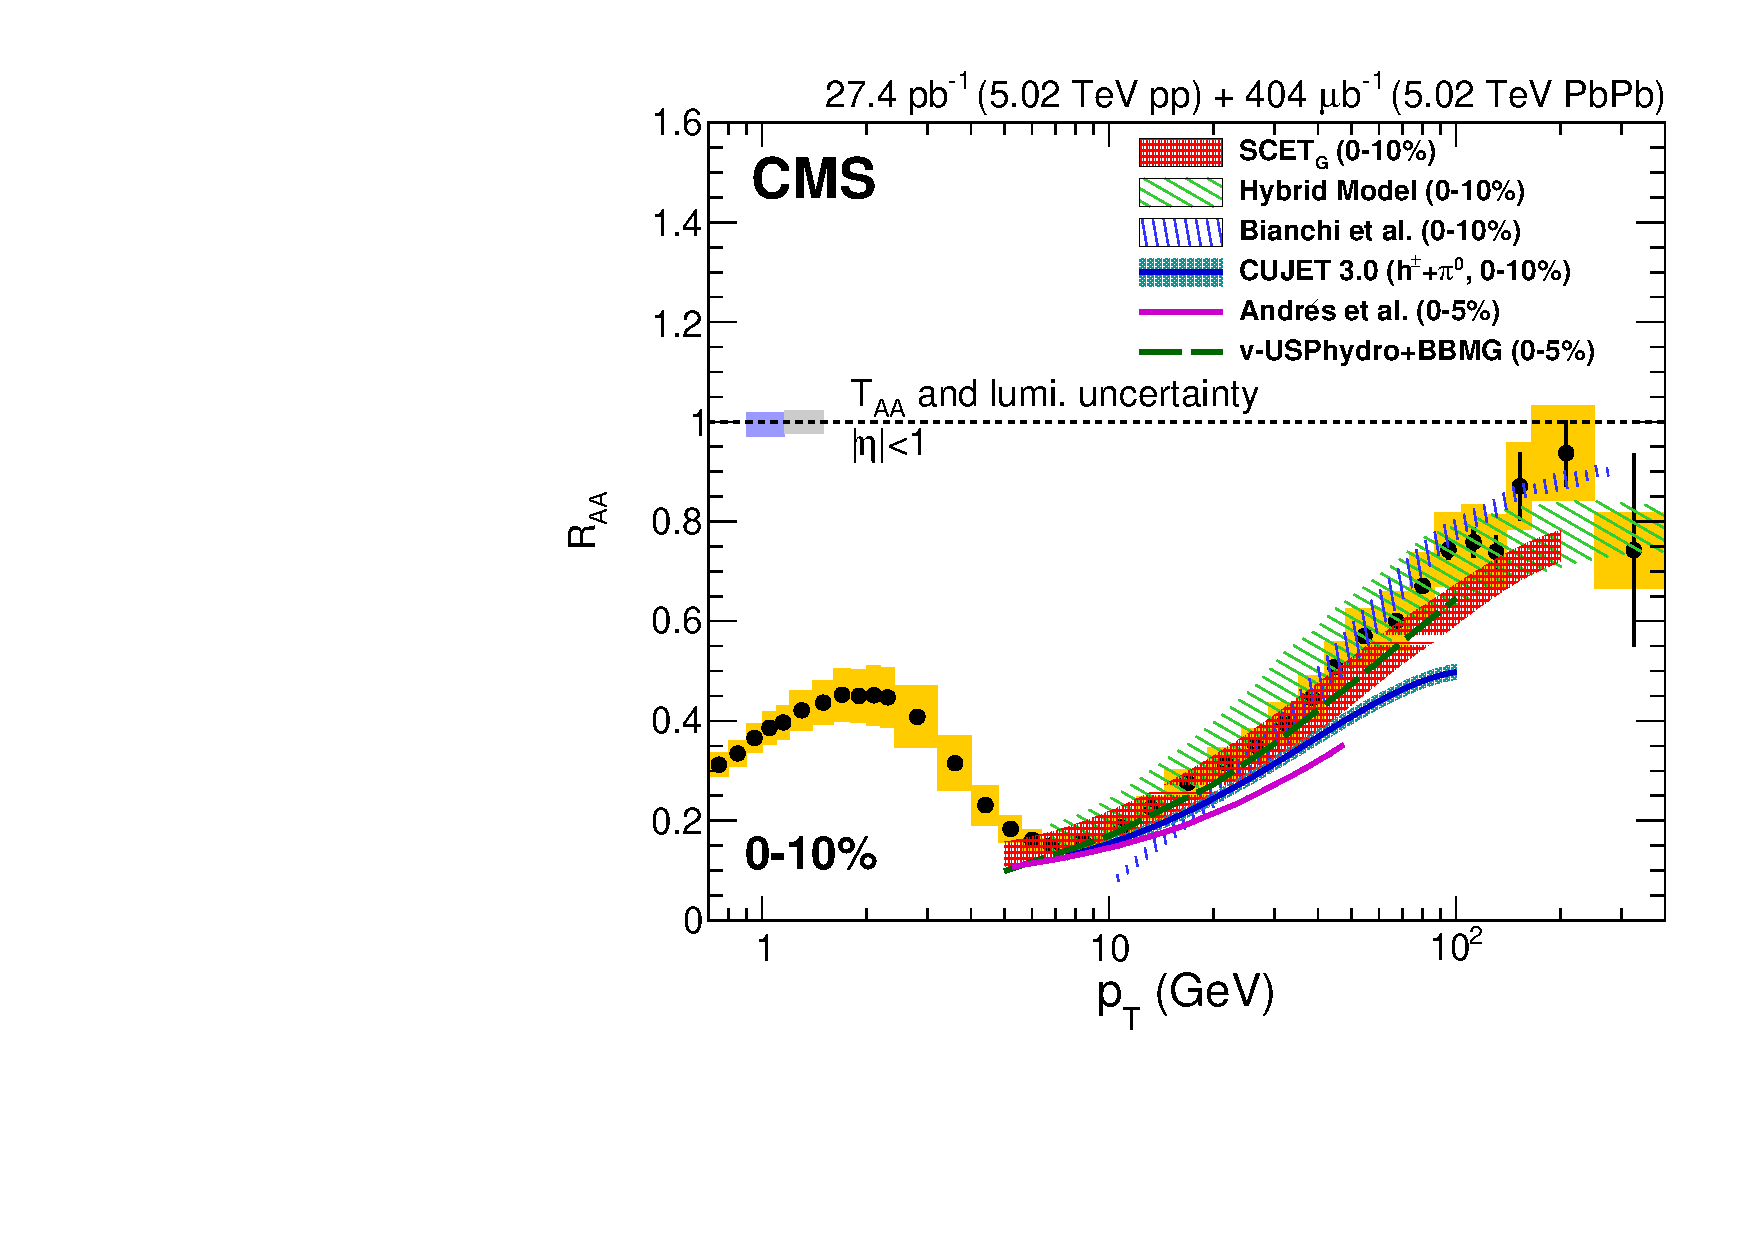
\includegraphics[width=0.7\textwidth]{figures/Theory/ChPart_Raa_CMS_Theory.pdf}
\caption[Model comparisons to charged particle $R_{AA}$ at 5.02 TeV]{Model comparisons to charged particle $R_{AA}$ in 0-10\% central PbPb data at 5.02 TeV from Ref.~\cite{Khachatryan:2016odn}.}
\label{fig:cms_chpart_raa_theory}
\end{center}
\end{figure}



\subsubsection{Quenching model comparisons: jet fragmentation functions}

\subsubsection{Quenching model comparisons: jet shapes}

\subsubsection{Quenching model comparisons: dijet asymmetry}
  
  
  
 \subsection{Theoretical motivations for detailed jet-track correlation studies}
 \label{sec:motivation}
 
  \subsubsection{Extenshion of jet shape measurements to large angles}
  
  \subsubsection{Detailed characterization of jet peak in separate dimensions $\Delta\eta$ and $\Delta\phi$}
  
  \subsubsection{Detailed characterization of leading and subleading jet peaks in dijet events}
  
  \subsubsection{Decomposition of contributions to momentum balance studies in dijet events}
  \label{sec:motivation_decomp}
  
  